\studynote{7}{Wed 30 Nov 2022 02:14}{Test for Limiting Distribution}

\section{Testing Limiting Distribution}

\subsection*{Motivation}

\textbf{The oversampling effect.} We need to numerically verify the limiting distribution of a random walk. We cannot sample from the limiting distribution directly, and instead can only sample from a location distribution after finitely many steps. Therefore, if we run a goodness-of-fit test directly between the empirical distribution and the hypothesized limiting distribution, the test will reject the null hypothesis $H_0$ after taking enough samples, even when $H_0$ is true.
For experiment outputs, see \verb|221119_ssrw_adapted_ks|.
This phenomenon introduces difficulty making precise statements of the limiting distribution. 

Therefore, we want to develop a method for testing limiting distributions. Our method should account for the difference between location distribution at step $m$ and the limiting distribution. Our method should consistently fail to reject $H_0$ when $H_0$ is true. Meanwhile, it should not make too much beta error, i.e. it should reject $H_0$ with high probability when $H_0$ is not true. 

\subsection*{Background}

Let $A_m$ be the location distribution of a random walk after $m$ steps.

Let $X_{m}^{(k)}, k = 1,\ldots, n$ be i.i.d samples from $A_m$. 

Let $S_{m,n}$ be the empirical cdf of the scaled scamples:
\[
S_{m,n}\left(x \right) =
\frac{1}{n} \sum_{k=1}^{n} \mathbf{1}\left( \frac{X_m^{(k)}}{\sigma \sqrt{m} } < x\right) 
.\] 

And let $F_m$ be cdf of $\frac{A_m}{\sigma \sqrt{m} }$, the scaled distribution at step $m$.

We assume the scaling term is $m^{-\frac{1}{2}}$ in this note, but this can be generalized.

By the Glivenko-Cantelli Theorem, as $n \to \infty $, $S_{m, n}\to F_m$ uniformly in distribution a.s.

We hypothesize that the random walk has limiting distribution $F_0$, that is, $F_m \to F_0$ uniformly in distribution as $m\to \infty$.

\subsection*{Development of The Test}

Our null hypothesis is
\[
	H_0: F_m \xRightarrow{m\to \infty } F_0
.\] 
Our alternative hypothesis is
\[
	H_A: F_m \text{ does not converge or } F_m \xRightarrow{m \to \infty } F' \not\equiv F_0 
.\] 





We define our test statistic to be
\[
	D_{m,n} = \operatorname{sup} _x \left| \tilde S_{m, n}(x) - F_0(x) \right| 
.\] 

We also define

\[
	K_{m, n} = \operatorname{sup} _x \left| \tilde S_{m, n}(x) - \tilde F_m(x) \right| 
.\] 

\[
	T_{m} = \operatorname{sup} _x \left| \tilde F_m(x) - F_0(x) \right| 
.\] 

$D_{m, n}, K_{m, n}$ and $T_m$ are $L_\infty $ distances between continuous cdfs on $[0,1]$, as depicted in the following diagram.
\begin{figure}[H]
	\centering
	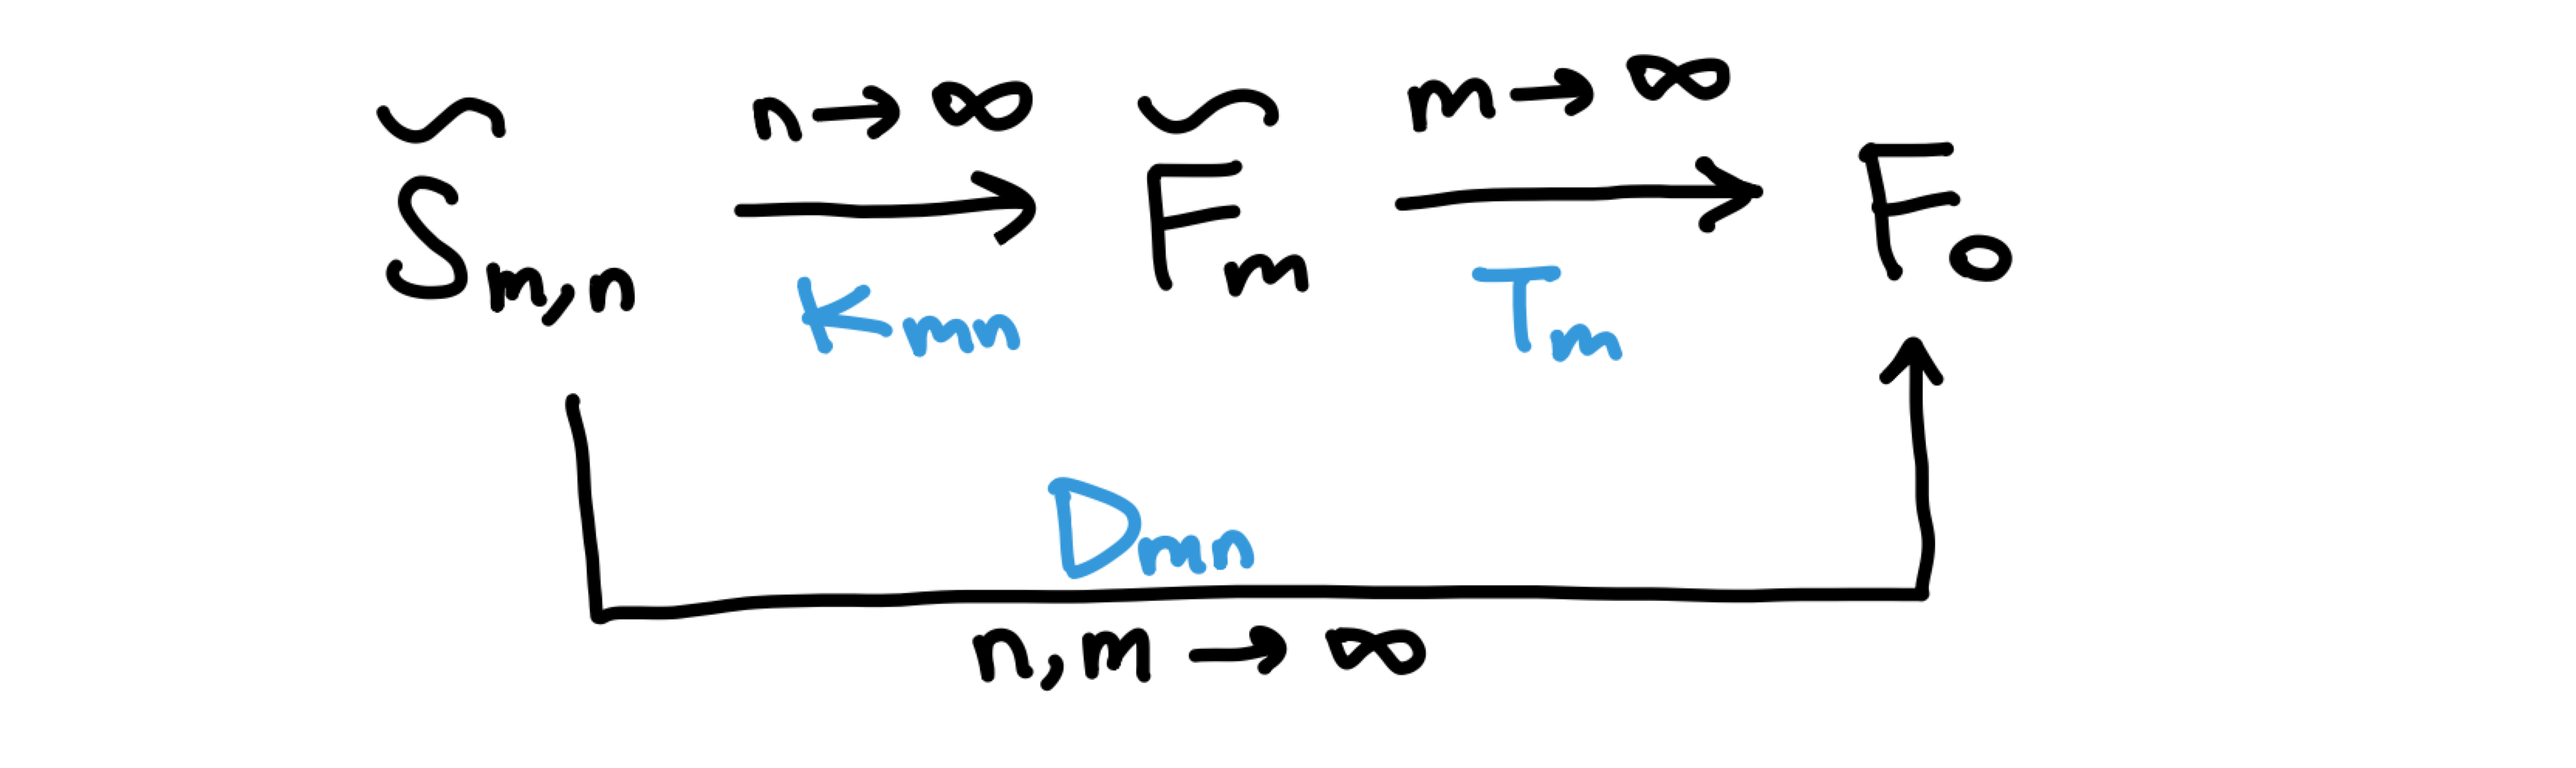
\includegraphics[width=0.8\textwidth]{figures/kstest-limits.png}
	\caption{}
	\label{fig:kstest-limits}
\end{figure}

We bound $K_{m, n}$ using Kolmogorov Theorem:
\[
	\operatorname{Pr} \left[ K_{m, n}< \frac{d}{\sqrt{n} }  | H_0\right] = L(d, n)
.\] 

We bound $T_m$ using Berry-Esseen Theorem:
\[
	T_{m} \le  0.4748 \frac{1}{\sqrt{m} }
.\] 

We can bound $D_{m, n}$ using triangle inequality:
\[
	K_{m, n} - T_{m} \le D_{m, n} \le  K_{m, n} + T_m
.\] 

Now we try to bound the probability that $D_{m, n} < \frac{v}{\sqrt{n} }$. For lower bound,
\begin{align*}
	&\operatorname{Pr} \left[ D_{m, n} < \frac{v}{\sqrt{n} }| H_0 \right]\\
	&\ge \operatorname{Pr} \left[ K_{m, n}+ T_m \le  \frac{v}{\sqrt{n} }| H_0 \right]  \\
	&\ge \operatorname{Pr} \left[ K_{m, n}< \frac{v}{\sqrt{n} } - 0.4748 \frac{1}{\sqrt{m} }|H_0 \right]  \\
	&= L\left( v - 0.4748 \sqrt{\frac{n}{m}}  \right)
.\end{align*}

Similarly, one can obtain an upper bound. Hence we can bound the cdf of $D_{m,n}$ conditioned on $H_0$ from above and below:
\[
	L\left( v - 0.4748 \sqrt{\frac{n}{m}}  \right) 
	\le \operatorname{Pr} \left[ D_{m, n} < \frac{v}{\sqrt{n} } | H_0 \right]
	\le L\left( v + 0.4748 \sqrt{\frac{n}{m}}  \right)
.\] 

Now the bound for $p\,$-value is given by
\[
	1 - L\left(v + 0.4748\sqrt{\frac{n}{m}}\right) \le  p \le 
	1 - L\left(v - 0.4748 \sqrt{\frac{n}{m}}\right) 
.\] 

For some fixed $\alpha$, we calculate the parameter  $v^*$ using
\[
	\alpha  = 1 - L\left(v^* + 0.4748\sqrt{\frac{n}{m}}\right)
\] 

The decision criterion is
\[
	D_{m, n} > \frac{v^*}{\sqrt{n} } = \frac{L^{-1} (1 - \alpha)}{\sqrt{n} } + 0.4748 \sqrt{\frac{1}{m}} 
\] 

or equivalently,
\[
	1 - L \left( D_{m, n}\sqrt{n} - 0.4748 \sqrt{\frac{n}{m}} \right)    < \alpha
.\] 

\subsection*{Application to SSRW and results}

Following are observations from applying this test to SSRW. For code and output, see \verb|221130_adapted_ks_1samp|.
\begin{enumerate}
	\item The oversampling effect vanishes: the test fails to reject every time, no matter how many samples we take.
	\item The test is very optimistic for $m < n$: the calculated $p$ value is almost always $1$.
	\item The test is still able to reject: when applied to a random walk generated using Cauchy distribution, the test consistently rejects the null hypothesis.
\end{enumerate}

\subsection*{Discussion}

Several problems still need to be addressed:
\begin{enumerate}
	\item The lower and upper bounds are not very tight when $m \approx n$. To obtain reasonably tight bound we $m$ bigger than $n$ by $1-2$ orders of magnitude. This is not a big problem in general, however, since we can pick $m \gg n$ if we want tighter bounds. I still wonder if the bound can be tightened further.
	\item 
\end{enumerate}


\subsection*{Further Steps}
`
\begin{enumerate}
	\item Develop a 2-sample version of this test.
	\item Apply to random walks with limiting distributions other than SSRW, to see if it works well in general.
\end{enumerate}

\section{Two-Sample Test}

In this research project, we are interested in specific types of reinforced random walks, which brings two complications:
\begin{enumerate}
	\item The limiting distribution is sometimes unknown. Therefore we can no longer have an explicit form of the limiting distribution and compare the walk to it using the 1 sample test.
	\item The steps are not i.i.d., so Berry-Esseen no longer applies. We can no longer control the speed of convergence of step-$m$ distribution $F_m$ to the limiting distribution $F_\infty $.
\end{enumerate}

To solve (1), developing a 2-sample test would be helpful. To deal with (2), we make assumptions of the rate of convergence $F_m \Rightarrow F_\infty$.

\subsection{Development of Two sample test}

Our null hypothesis is
\[
	H_0: \begin{cases}
	F_m \xRightarrow{m\to \infty } F_\infty \\
	F'_m \xRightarrow{m\to \infty } F_\infty \\
	\end{cases}
	\text{ for some cdf }F_\infty 
.\] 

We define our test statistic to be
\[
	D_{m, n} = \operatorname{sup}_x \left| \tilde{S}_{m, n}(x) - \tilde{S}'_{m, n}(x)  \right| 
.\] 

We also define
\[
	K_{m, n} = \operatorname{sup}_x \left| \tilde{S}_{m, n}(x) - \tilde{F}_{m}(x)  \right| 
.\]
\[
	K'_{m, n} = \operatorname{sup}_x \left| \tilde{S}'_{m, n}(x) - \tilde{F}_{m}(x)  \right| 
.\]
\[
	T_{m} = \operatorname{sup}_x \left| \tilde{F}_{m}(x) - {F}_\infty (x)  \right| 
.\]
\[
	T'_{m} = \operatorname{sup}_x \left| \tilde{F'}_{m}(x) - {F'}_\infty (x)  \right| 
.\]

$K$ and  $K'$ are controlled by Kolmogorov Theorem. Now by using triangle inequality, we obtain the following:
\[
	|K_{m,n} - K'_{m,n}| \le |D_{m, n} - \frac{\Delta}{\sqrt{n} } | \le K_{m, n} + K'_{m,n}
.\] 
where $\Delta:= \sqrt{n} \operatorname{sup}_x |F_m(x) - F'_m(x)|$.

Now we obtain a concentration bound for $|D_{m, n} - \Delta |$:
 \[
	 \operatorname{Pr} \left[ K_{m, n} + K'_{m,n} < \frac{d}{\sqrt{n} }| H_0 \right] \le 
	 \operatorname{Pr} \left[ |D_{m, n} - \frac{\Delta}{\sqrt{n} }| < \frac{d}{\sqrt{n} }| H_0 \right] \le 
	 \operatorname{Pr} \left[ |K_{m,n} - K'_{m,n}| < \frac{d}{\sqrt{n} }| H_0 \right] 
.\] 

Write as convolution and apply Kolmogorov Theorem:
\begin{equation}
	\label{eqn:2samp-bounds}
	 \int _0^d L(d-a, n) dL(a, n) \le 
	 \operatorname{Pr} \left[ |D_{m, n} - \frac{\Delta}{\sqrt{n} }| < \frac{d}{\sqrt{n} }| H_0 \right] \le 
	\int _0^\infty  \int_{a - d}^{a + d} dL(b, n) dL(a, n)
.\end{equation}


where $a$ and $b$ are variables for integration. The left hand side is $0$ when $d < 0$.

For simplicity of notation, we write the inequality above as
\begin{equation}
	 A(d,n) \le 
	 \operatorname{Pr} \left[ |D_{m, n} - \frac{\Delta}{\sqrt{n} }| < \frac{d}{\sqrt{n} }| H_0 \right] \le 
	B(d, n) 
.\end{equation}

After some manipulations,
\begin{equation}
	 A(d - \Delta, n) \le 
\operatorname{Pr} \left[ D_{m, n}  < \frac{d}{\sqrt{n} }| H_0 \right] \le 
1 - A(\Delta - d, n)
.\end{equation} 

Now we can proceed in the same way as 1 sample test.

\subsubsection*{Implementation and Result}
Evaluated bounds in \eqref{eqn:2samp-bounds} numerically. We have two issues:
\begin{itemize}
	\item The bounds are extremely loose, to ensure a $0.95$ upper bound, the lower bound would be very close to $0$. Even worse, \eqref{eqn:2samp-bounds} is still a bound for 
		$ \operatorname{Pr} \left[ |D_{m, n} - \frac{\Delta}{\sqrt{n} }| < \frac{d}{\sqrt{n} }| H_0 \right] $
	, to obtain a bound for 
$\operatorname{Pr} \left[ D_{m, n}  < \frac{d}{\sqrt{n} }| H_0 \right] $
we would need to get even looser.
	\item The bounds are inefficient to compute. Computing this graph takes $\approx 5$ minutes.
\end{itemize}

\subsubsection*{Discussion}
We still have the following problems
\begin{enumerate}
	\item No effective way to control $\Delta$. For application purposes we may assume $\Delta$ goes to $0$ in $n^{-1} $ rate and choose an appropriate constant such that $\Delta = o(n^{-1} )$.
	\item No control of beta error, similar to the 1 sample case.
\end{enumerate}
